\documentclass[11pt,a4paper]{article}

% ---------------------------------------------------------------------------
% Linear-size autocatalytic sets are asymptotically absent in the sparse
% binary polymer model.
%
% Author metadata: set the macros below before submission.
% ---------------------------------------------------------------------------
\newcommand{\PaperAuthor}{Anonymous manuscript}
\newcommand{\PaperAffiliation}{}
\newcommand{\PaperDate}{14 September 2026}

\usepackage[T1]{fontenc}
\usepackage[utf8]{inputenc}
\usepackage{lmodern}
\usepackage{microtype}
\usepackage[a4paper,margin=1.05in]{geometry}
\usepackage{amsmath,amssymb,amsthm}
\usepackage{booktabs}
\usepackage{array}
\usepackage{enumitem}
\usepackage{xcolor}
\usepackage{tikz}
\usetikzlibrary{arrows.meta,positioning,calc,fit,backgrounds}
\renewcommand{\topfraction}{0.9}
\renewcommand{\textfraction}{0.05}
\renewcommand{\floatpagefraction}{0.75}
\usepackage[obeyspaces,spaces]{url}
\usepackage[numbers,sort&compress]{natbib}
\usepackage[colorlinks=true,linkcolor=blue!55!black,citecolor=blue!55!black,urlcolor=blue!55!black]{hyperref}
\hypersetup{pdftitle={Linear-size autocatalytic sets are asymptotically absent in the sparse binary polymer model},
 pdfauthor={\PaperAuthor},
 pdfsubject={Minimum size of RAFs in the sparse catalysis polymer model of Hordijk and Steel},
 pdfkeywords={autocatalytic sets, RAF theory, binary polymer model, sparse catalysis, random reaction networks, formal verification}}

\providecommand{\doi}[1]{}
\renewcommand{\doi}[1]{\href{https://doi.org/#1}{\nolinkurl{doi:#1}}}

\setlist{itemsep=2pt,topsep=3pt}
\setlength{\emergencystretch}{1.5em}

\theoremstyle{plain}
\newtheorem{theorem}{Theorem}[section]
\newtheorem{proposition}[theorem]{Proposition}
\newtheorem{lemma}[theorem]{Lemma}
\newtheorem{corollary}[theorem]{Corollary}
\theoremstyle{definition}
\newtheorem{definition}[theorem]{Definition}
\newtheorem{example}[theorem]{Example}
\theoremstyle{remark}
\newtheorem{remark}[theorem]{Remark}
\newtheorem{question}[theorem]{Question}

\DeclareUrlCommand\lean{\urlstyle{tt}}

\newcommand{\cl}{\operatorname{cl}}
\newcommand{\Nat}{\mathbb N}
\newcommand{\Real}{\mathbb R}
\newcommand{\cA}{\mathcal A}
\newcommand{\cR}{\mathcal R}
\newcommand{\cX}{\mathcal X}
\newcommand{\cP}{\mathcal P}
\newcommand{\cH}{\mathcal H}
\newcommand{\eend}{\operatorname{end}}
\newcommand{\Uni}{\operatorname{U}}
\newcommand{\ee}{\mathrm e}

\title{Linear-size autocatalytic sets are asymptotically absent\\ in the sparse binary polymer model}
\author{\PaperAuthor\\ \PaperAffiliation}
\date{\PaperDate}

\begin{document}
\maketitle

\begin{abstract}
In the binary polymer model of Kauffman, molecules are bit strings of length at most $n$, reactions are ligations and their reverse cleavages, and a random catalysis assignment decides which molecules catalyse which reactions. Hordijk and Steel (\emph{J.\ Math.\ Chem.}, 2016) introduced a \emph{sparse} catalysis law, in which a molecule is active with a small probability and an active molecule catalyses each reaction independently with probability $1/n$, and showed that when the expected number of reactions catalysed per molecule is $\lambda n$ for a large fixed $\lambda$, the system contains a reflexively autocatalytic and food-generated set (RAF) with fewer than $2\lambda n^2$ reactions with probability close to one. They asked whether the quadratic size can be reduced to linear, and in particular whether a single molecule is likely to catalyse a set of reactions that suffices to construct that molecule once cleavage reactions are allowed. We answer both questions negatively. For every fixed food horizon, every fixed nonnegative intensity $\lambda$ and every fixed constant $C$, the probability that the model contains a nonempty RAF with at most $Cn$ reversible reactions tends to zero as $n\to\infty$, at rate $O(1/n)$; the probability that some molecule catalyses a self-constructing set tends to zero as well, cleavage included. The proof separates two regimes by the number of catalysts a RAF uses. Boundedly many catalysts are excluded by a productive-prefix argument whose constants do not depend on $n$. Many catalysts are excluded by a counting lemma of independent interest: the number of $m$-reaction sets that can be built productively from the food, multiplied by $m!$, is at most $\big((f+3m)^2+n(f+3m)\big)^m$, where $f$ is the food size. The factorial comes from an injective acyclic dependency encoding of arbitrarily labelled constructions and is exactly the entropy saving that the sparsity of active molecules cannot otherwise absorb. Consequences include the divergence of the minimum RAF size relative to $n$, the divergence of the minimum catalyst count, conditional versions on RAF existence, and a superlinear-to-quadratic window for the minimum RAF size in the regime of Hordijk and Steel. The main theorem, its constituent estimates and all stated consequences are verified in Lean~4 against the literal split-position model.
\end{abstract}

\noindent\textbf{Keywords.} autocatalytic sets; RAF theory; binary polymer model; sparse catalysis; random reaction networks; origin of life; formal verification.

\medskip
\noindent\textbf{MSC 2020.} 92E20, 60C05, 05A16, 92D15, 68V20.

\section{Introduction}\label{sec:intro}

A reflexively autocatalytic and food-generated set, or RAF, is a finite combinatorial abstraction of a collectively self-sustaining chemistry: a set of reactions all of whose reactants can be built from a freely available \emph{food} set by reactions of the set, and each of whose reactions is catalysed by a molecule that is food or is produced by the set \cite{hordijk2004detecting,steel2019autocatalytic}. The notion descends from Kauffman's autocatalytic sets of proteins \cite{kauffman1986autocatalytic,kauffman1993origins}, and the \emph{binary polymer model} that Kauffman proposed to study them remains the standard random model. Molecules are the bit strings of length at most $n$; food consists of all strings of length at most a fixed small $t$; the reactions are all ligations $u+v\to uv$ together with their reverse cleavages; and catalysis is assigned at random. When each molecule catalyses each reaction independently with the same probability (the \emph{uniform} law), bounds on the RAF probability initiated by Kauffman and Steel \cite{kauffman1986autocatalytic,steel2000emergence} were sharpened by Mossel and Steel \cite{mossel2005random}, who showed that RAFs appear precisely when the expected number $f$ of reactions catalysed per molecule grows linearly with $n$; at this level of catalysis the RAFs that first appear are of exponential size \cite{hordijk2011required,hordijk2016variable}.

Hordijk and Steel \cite{hordijk2016variable,hordijk2017chasing} then asked how these conclusions depend on the \emph{distribution} of catalytic activity across molecule types, motivated by the observation that real metabolic networks are far from uniform. Among the laws they analysed is the \emph{sparse} law: each molecule type independently is \emph{active} with probability $p$, and an active molecule catalyses each reaction independently with probability $1/n$, so that $f=p|\cR_n|/n$. They proved that the linear threshold $f\asymp n$ for RAF emergence is universal across such distribution-based laws, but that the size of the RAFs that appear is not. In the sparse law with $f=\lambda n$ and $\lambda$ large, Chernoff's bound gives at most $2\lambda n$ active molecules with high probability, and a chain of fewer than $n$ ligations reaches every molecule, so a RAF with fewer than $2\lambda n^2$ reactions exists with probability at least $1-\varepsilon-o(1)$ \cite[Corollary~2]{hordijk2016variable}. Their concluding section \cite[Section~7]{hordijk2016variable} poses the problem this paper resolves. Having shown that the sparse model is likely to have RAFs of at most quadratic size when RAFs first appear, they ask whether this can be improved to order $n$, and in particular whether it is likely that a single molecule type catalyses a sequence of reactions sufficient to construct that molecule. They note that a simple argument rules the latter out asymptotically when only ligation reactions are used, but that ``the situation is less clear without this restriction'', that is, once cleavage reactions are allowed.

\subsection{Main result}

We work with the literal reversible split-position binary polymer model: a \emph{channel} is a product word $w$ together with a split position, its two orientations are the ligation of the two factors and the cleavage of the product, and both orientations are catalysed by the same random coordinate, exactly as in the bidirectional convention of \cite{hordijk2016variable}. The sparse law is parametrised so that the expected number of channels catalysed by a molecule is $\lambda n$ (Section~\ref{sec:model}).

\begin{theorem}[absence of linear-size RAFs]\label{thm:main}
Fix a food horizon $t\in\Nat$, an intensity $\lambda\ge 0$ and a real constant $C$. In the sparse binary polymer model with maximum length $n$,
\begin{equation}\label{eq:main}
\Pr\bigl\{\exists\,T:\ T\text{ is a nonempty RAF and }|T|\le Cn\bigr\}\longrightarrow 0\qquad(n\to\infty).
\end{equation}
Moreover the probability is $O(1/n)$.
\end{theorem}

All three parameters are fixed before $n$ tends to infinity. In particular no choice of a larger fixed intensity produces RAFs within a fixed linear budget with non-vanishing probability, so the quadratic bound of \cite[Corollary~2]{hordijk2016variable} cannot be improved to linear in the sense they ask (Corollary~\ref{cor:negation}). The theorem covers every number of catalysts, both orientations of every channel, and the actual dependence between catalytic events that share an active molecule. The single-molecule question is answered by a short separate argument that also handles cleavage (Proposition~\ref{prop:single}), and the same method shows that the minimum number of catalysts used by any RAF diverges (Theorem~\ref{thm:rank}).

\subsection{Method}

Let $T$ be a RAF and let $K$ be a set of molecules, one catalyst per channel, chosen inside the food closure of $T$. Every member of $K$ is active, an event of probability $p_n=\lambda n^2/|\cR_n|\approx\lambda n/|\cX_n|$ per molecule, and each channel of $T$ is covered by a conditional coordinate of probability $1/n$. Two effects compete. Few catalysts are cheap in activity but must cover many channels each; many catalysts cover cheaply but are individually rare. The proof treats the two regimes separately, and a fixed cutoff on $|K|$ that does not depend on $n$ separates them (Figure~\ref{fig:architecture}).

For a bounded number $k$ of catalysts we use a \emph{productive-prefix} argument (Section~\ref{sec:bounded}). A catalyst that is not itself reachable by short constructions forces the RAF to contain a productive construction of depth $d$ from the food, and the number of such depth-$d$ constructions is bounded independently of $n$ because a depth-$d$ construction only sees molecules of length at most $t2^d$. Choosing $d=k+1$ leaves the factor $(|\cX_n|p_n/n)^k/n\to 0$.

For many catalysts the union over catalyst sets is too expensive and we must instead count the constructions themselves. The core of the paper is the following deterministic statement (Lemma~\ref{lem:factorial}). Let $\cA_m$ be the family of $m$-channel sets that admit a \emph{productive program} from the food, that is, an ordering in which every channel is enabled in one of its orientations when it fires and adds at least one new molecule. Then
\begin{equation}\label{eq:factorial-intro}
|\cA_m|\cdot m!\ \le\ \bigl((f+3m)^2+n(f+3m)\bigr)^m ,\qquad f=|F|.
\end{equation}
Each channel of a labelled construction can be described by an \emph{instruction} that refers to its inputs either as food molecules or as endpoints of earlier channels, and the resulting acyclic code determines the labelled channel assignment uniquely. The factorial counts the $m!$ arbitrary labellings of one support. It is \emph{not} the number of productive orders of a support, which may be as small as one; a single productive order merely certifies that the code is acyclic. Under a linear budget $m\le Cn$ the factorial exactly cancels the $n^m$ from the cleavage split positions and leaves $|\cA_m|\le (Dn)^m$ with $D$ depending only on $t$ and $C$. The $n^{-m}$ from the conditional coordinates then cancels the $n^m$ from the support count, and the activity factor $((f+3Cn)p_n)^k$ with $k$ large is exponentially small (Section~\ref{sec:large}).

A RAF need not be a productive program: it may contain channels that no construction ever uses. A saturated productive extraction (Lemma~\ref{lem:saturated}) replaces the RAF by a productive sub-support whose final state contains the entire original food closure, so every original catalyst is still available and every extracted channel is still covered. This step is what allows the support count to control arbitrary RAFs.

\subsection{Formal verification}

The main theorem, the two probability estimates, the factorial count, the saturated extraction, the single-catalyst statement and all consequences in Section~\ref{sec:consequences} have been checked in Lean~4 \cite{demoura2021lean4,mathlib2020} against the literal source model, with the sparse law realised as an infinite product measure. The verified statements depend only on the standard axioms of Lean's kernel. Section~\ref{sec:formal} gives the concordance between the paper and the formal development and states exactly what is cited rather than proved.

\subsection{Organisation}

Section~\ref{sec:model} defines the model and records the counts and parameters used throughout. Section~\ref{sec:results} states all results. Section~\ref{sec:programs} develops productive programs, saturated extraction and prefix counting. Section~\ref{sec:bounded} proves the bounded-rank theorem, Section~\ref{sec:large} the factorial count and the large-rank tail, and Section~\ref{sec:proof} assembles the main theorem with its rate. Section~\ref{sec:single} treats the single-molecule question, Section~\ref{sec:consequences} the consequences, Section~\ref{sec:formal} the verification, and Section~\ref{sec:discussion} the scope of the result and open problems.

\begin{figure}[t]
\centering
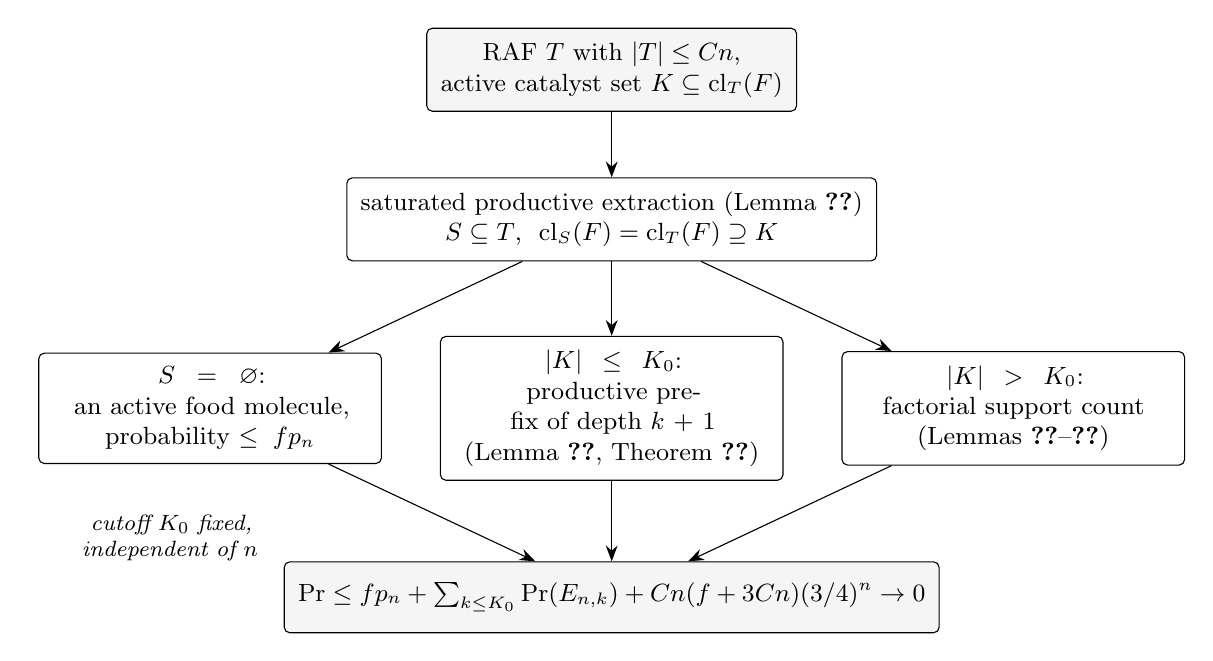
\begin{tikzpicture}[
  box/.style={draw,rounded corners=2pt,align=center,inner sep=5pt,font=\small,minimum height=9mm},
  lab/.style={font=\footnotesize\itshape},
  >={Stealth[length=2mm]}]
\node[box,fill=gray!8] (raf) at (0,0) {RAF $T$ with $|T|\le Cn$,\\ active catalyst set $K\subseteq\cl_T(F)$};
\node[box] (sat) at (0,-1.9) {saturated productive extraction (Lemma~\ref{lem:saturated})\\ $S\subseteq T$, \ $\cl_S(F)=\cl_T(F)\supseteq K$};
\node[box,text width=40mm] (empty) at (-5.1,-4.3) {$S=\varnothing$:\\ an active food molecule,\\ probability $\le f p_n$};
\node[box,text width=40mm] (small) at (0,-4.3) {$|K|\le K_0$:\\ productive prefix of depth $k+1$\\ (Lemma~\ref{lem:depth}, Theorem~\ref{thm:rank})};
\node[box,text width=40mm] (big) at (5.1,-4.3) {$|K|>K_0$:\\ factorial support count\\ (Lemmas~\ref{lem:factorial}--\ref{lem:tail})};
\node[box,fill=gray!8] (sum) at (0,-6.7) {$\Pr\le f p_n+\sum_{k\le K_0}\Pr(E_{n,k})+Cn(f+3Cn)(3/4)^n\to 0$};
\draw[->] (raf) -- (sat);
\draw[->] (sat) -- (empty);
\draw[->] (sat) -- (small);
\draw[->] (sat) -- (big);
\draw[->] (empty) -- (sum);
\draw[->] (small) -- (sum);
\draw[->] (big) -- (sum);
\node[lab,text width=34mm,align=center] at (-5.6,-5.95) {cutoff $K_0$ fixed,\\ independent of $n$};
\end{tikzpicture}
\caption{Architecture of the proof of Theorem~\ref{thm:main}. A fixed catalyst cutoff separates the productive-prefix estimate, which has no size restriction, from the factorial support count, which uses the linear budget.}
\label{fig:architecture}
\end{figure}

\section{The model}\label{sec:model}

\subsection{Molecules, channels and closure}

Let $\cX_n$ be the set of nonempty binary words of length at most $n$. A \emph{channel} is a pair $(w,i)$ with $w\in\cX_n$ and $1\le i<|w|$; writing $w=uv$ with $|u|=i$, the channel has the two orientations
\[
u+v\ \longrightarrow\ w\quad(\text{ligation}),\qquad w\ \longrightarrow\ u+v\quad(\text{cleavage}),
\]
and its \emph{endpoints} are $\eend(w,i)=\{u,v,w\}$. Let $\cR_n$ be the set of channels. Distinct split positions of the same word are distinct channels even when they produce the same unordered factor pair, and equal factors are allowed; this is the literal reaction catalogue of the binary polymer model, in which each ligation and its reverse cleavage are counted as one bidirectional reaction \cite{hordijk2016variable}. Summing $2^\ell$ words with $\ell-1$ split positions over lengths $\ell\le n$,
\begin{equation}\label{eq:counts}
N_n:=|\cX_n|=2^{n+1}-2,\qquad R_n:=|\cR_n|=(n-2)2^{n+1}+4\quad(n\ge2),
\end{equation}
so that $R_n/(nN_n)\to1$, in agreement with the relation $|\cR_n|\sim n|\cX_n|$ of \cite{mossel2005random}. We shall also use $R_n\ge 2^n$ for $n\ge 2$.

The food set is $F=\cX_t$ for a fixed horizon $t$ (the literature instance is $t=2$), and $f:=|\cX_t|=2^{t+1}-2$. We assume $n\ge\max\{2,t\}$, which is harmless for limits.

For a set $T\subseteq\cR_n$ of channels and a set $A\subseteq\cX_n$ of available molecules, a channel is \emph{enabled} at $A$ if both its factors lie in $A$ or its product lies in $A$. The \emph{food closure} $\cl_T(F)$ is the least set containing $F$ and closed under both orientations of every channel of $T$; concretely it is the union of the increasing sequence $A_0=F$, $A_{j+1}=A_j\cup\bigcup_{r\in T,\ r\text{ enabled at }A_j}\eend(r)$. The set $T$ is \emph{food-generated} if every channel of $T$ has all its endpoints in $\cl_T(F)$, equivalently is enabled there.

\begin{definition}[RAF]\label{def:raf}
Given a catalysis relation $\mathsf{C}\subseteq\cX_n\times\cR_n$, a set $T\subseteq\cR_n$ is a \emph{RAF} if it is nonempty, food-generated, and every $r\in T$ has a catalyst $x\in\cl_T(F)$ with $(x,r)\in\mathsf{C}$.
\end{definition}

This is the reversible RAF notion of \cite{hordijk2016variable}: catalysis is assigned to the channel, so a catalyst of $(w,i)$ catalyses both the ligation and the cleavage, and a catalyst may be produced by the set rather than being available before the construction starts.

\subsection{The sparse catalysis law}

For each molecule $x\in\cX_n$ let $A_x$ be a Bernoulli variable of parameter $p_n$ (\emph{activity}), and for each pair $(x,r)\in\cX_n\times\cR_n$ let $B_{x,r}$ be a Bernoulli variable of parameter $q_n$ (\emph{conditional channel bit}). All these variables are independent. The random catalysis relation is
\[
(x,r)\in\mathsf{C}\quad\Longleftrightarrow\quad A_x=1\ \text{and}\ B_{x,r}=1 .
\]
This is the sparse law of \cite[Section~2]{hordijk2016variable}: with probability $p_n$ a molecule ``catalyzes each reaction independently with probability $1/n$'', otherwise it catalyses nothing. Following \cite{hordijk2016variable} we normalise the expected number of channels catalysed by a molecule, $f_n=p_nq_nR_n$, to be $\lambda n$:
\begin{equation}\label{eq:parameters}
q_n=\frac1n,\qquad p_n=\frac{\lambda n^2}{R_n},\qquad p_nq_nR_n=\lambda n .
\end{equation}
For fixed $\lambda\ge0$ we have $p_n\le\lambda n^2/2^n\to0$, so $p_n\le1$ for all large $n$; the formal model clips $p_n$ to $[0,1]$ at the finitely many small $n$ where the formula exceeds one, which does not affect any limit. We record the consequences of \eqref{eq:counts}--\eqref{eq:parameters} that are used below:
\begin{equation}\label{eq:asymptotics}
np_n\to0,\qquad \frac{N_np_n}{n}=\frac{\lambda nN_n}{R_n}\to\lambda,\qquad (f+3Cn)\,p_n\le\Bigl(\tfrac{9}{16}\Bigr)^n\ \text{for all large }n .
\end{equation}
The last statement holds because $(f+3Cn)p_n\le\lambda(fn^2+3Cn^3)/2^n$ and a fixed polynomial is eventually dominated by $(9/8)^n$.

The events $(x,r)\in\mathsf{C}$ and $(x,r')\in\mathsf{C}$ for $r\ne r'$ are positively correlated, since both require $A_x=1$; \cite{hordijk2016variable} point out that this correlation is exactly what distinguishes distribution-based laws from the uniform law. All probability estimates below are stated and proved for the product law of the underlying variables $(A_x)$ and $(B_{x,r})$, and none replaces the sparse law by independent catalysis marginals.

\subsection{Notation}

Throughout, $\lambda\ge0$, $t$ and $C$ are fixed. We write $p=p_n$ and $q=q_n$ when $n$ is clear. For a finite set $S$ of channels its \emph{universe} is $\Uni(S)=F\cup\bigcup_{r\in S}\eend(r)$, of cardinality at most $f+3|S|$.

\section{Statement of results}\label{sec:results}

Let $L_n(C)$ be the event in \eqref{eq:main}, that some nonempty RAF has at most $Cn$ channels. A \emph{catalyst cover} of a RAF $T$ is a set $K\subseteq\cl_T(F)$ of molecules such that every channel of $T$ is catalysed by a member of $K$; its size is the \emph{rank} of the cover. Let $E_{n,k}$ be the event that some nonempty food-generated channel set has an active catalyst cover of rank exactly $k$ whose members are all reachable, i.e.\ lie in its food closure. (Unused members of a cover may be deleted, so ``rank at most $k$'' and ``rank exactly $k'$ for some $k'\le k$'' describe the same event.)

\begin{theorem}[bounded catalyst rank]\label{thm:rank}
For every fixed $k\ge1$, $\Pr(E_{n,k})=O(1/n)$. Consequently, for every fixed $K$, the probability that some RAF, of any size, has a catalyst cover of rank at most $K$ tends to zero.
\end{theorem}

\begin{proposition}[single-molecule self-construction]\label{prop:single}
Let $\mathrm{Self}_n$ be the event that some molecule $x$ catalyses every channel of a nonempty food-generated set $T$ with $x\in\cl_T(F)$. Then, cleavage included,
\[
\Pr(\mathrm{Self}_n)\ \le\ |\cX_{2t}|\,p_n+N_nR_{2t}R_{4t}\,p_nq_n^2\ \longrightarrow\ 0 .
\]
\end{proposition}

\begin{corollary}[negation of the linear-size assertion]\label{cor:negation}
For every fixed food horizon $t$, the following statement is false: for every $\varepsilon>0$ there exist $\lambda\ge0$ and $C\ge0$ such that $\Pr(L_n(C))\ge1-\varepsilon$ for all large $n$.
\end{corollary}

\begin{corollary}[rate]\label{cor:rate}
For fixed $t$, $\lambda\ge0$ and integer $C\ge0$ there is a constant $A<\infty$ such that, for all large $n$,
\begin{equation}\label{eq:rate}
\Pr(L_n(C))\ \le\ \frac{A}{n}+Cn\,(f+3Cn)\Bigl(\tfrac34\Bigr)^n .
\end{equation}
An admissible $A$ is given in \eqref{eq:A}.
\end{corollary}

Let $M_n$ be the minimum number of channels of a nonempty RAF, and $J_n$ the minimum rank of an active reachable catalyst cover of a RAF; both are $+\infty$ when no RAF exists. Let $G_n$ be the event that a RAF exists.

\begin{corollary}[minima and conditioning]\label{cor:minima}
For every fixed real $C$ and integer $K$, $\Pr(M_n\le Cn)\to0$ and $\Pr(J_n\le K)\to0$. If $\liminf_n\Pr(G_n)>0$, then also $\Pr(M_n\le Cn\mid G_n)\to0$ and $\Pr(J_n\le K\mid G_n)\to0$.
\end{corollary}

\begin{corollary}[superlinear-to-quadratic window]\label{cor:window}
In the regime of \cite[Corollary~2]{hordijk2016variable}, i.e.\ $t$ fixed, $0<\varepsilon<1$, and $\lambda$ fixed and large enough that the RAF probability bound of \cite[Theorem~1]{hordijk2016variable} is at least $1-\varepsilon$, for every fixed $C$
\[
\Pr\bigl(Cn<M_n<2\lambda n^2\bigr)\ \ge\ 1-\varepsilon-o(1).
\]
\end{corollary}

The quadratic upper event in Corollary~\ref{cor:window} is a cited input; only the subtraction of the vanishing linear event is proved here. No lower bound of order $n^2$ and no concentration of $M_n$ at a particular intermediate scale is claimed; see Section~\ref{sec:discussion}.

\section{Productive programs}\label{sec:programs}

\subsection{Programs and saturated extraction}

Fix $n$ and $t$. A channel $r$ is \emph{productive} at an available set $A$ if it is enabled at $A$ and $\eend(r)\not\subseteq A$. Firing $r$ at $A$ yields $A\cup\eend(r)$; since one side of $r$ was already in $A$, this is exactly the closure update in the enabled orientation. A \emph{productive program} from $A$ with allowed set $U$ is a finite sequence $r_1,\dots,r_m$ of channels of $U$ such that each $r_j$ is productive at $A_{j-1}$, where $A_0=A$ and $A_j=A_{j-1}\cup\eend(r_j)$; its \emph{support} is $\{r_1,\dots,r_m\}$ and its \emph{final state} is $A_m$.

\begin{lemma}\label{lem:program-basic}
In a productive program the channels $r_1,\dots,r_m$ are pairwise distinct, $|A_j|\ge|A|+j$, and $A_m=A\cup\bigcup_j\eend(r_j)$. Every molecule of $A_m$ has length at most $L\,2^m$ if every molecule of $A$ has length at most $L$.
\end{lemma}

\begin{proof}
After $r_j$ fires, all its endpoints are available, so $r_j$ is never productive again. Each firing adds at least one molecule, and adds exactly the endpoints of the fired channel. A ligation at most doubles the maximum length present and a cleavage does not increase it.
\end{proof}

\begin{lemma}[saturated extraction]\label{lem:saturated}
For every finite $T\subseteq\cR_n$ there is a productive program from $F$ with support $S\subseteq T$ whose final state equals $\cl_T(F)$. In particular $\cl_T(F)=\Uni(S)$ and $|\cl_T(F)|\le f+3|S|$.
\end{lemma}

\begin{proof}
Starting from $F$, fire any productive channel of $T$ while one exists. The available set strictly increases inside the finite set $\cX_n$, so the procedure stops, at a state $B$. Every molecule added along the way lies in $\cl_T(F)$, so $B\subseteq\cl_T(F)$. At $B$ no channel of $T$ is productive: every channel of $T$ enabled at $B$ has all its endpoints in $B$. Hence $B$ is closed under both orientations of every channel of $T$ and contains $F$, so $\cl_T(F)\subseteq B$. The formula for $B$ and the cardinality bound are Lemma~\ref{lem:program-basic}.
\end{proof}

Now let $T$ be a RAF and choose for every channel one catalyst in $\cl_T(F)$; let $K$ be the set of chosen molecules. Every member of $K$ is active and $K\ne\varnothing$. Apply Lemma~\ref{lem:saturated} to $T$ and let $S$ be the extracted support. Since $\cl_S(F)=\cl_T(F)\supseteq K$, every channel of $S$ is still covered by $K$ and every member of $K$ is still reachable from $S$. Two cases arise.
\begin{itemize}
\item If $S\ne\varnothing$, then $S$ is itself a RAF with $|S|\le|T|$: its productive program supplies food generation and its final state $\Uni(S)$ supplies the catalysts.
\item If $S=\varnothing$, then $\cl_T(F)=F$, so a catalyst of any channel of the nonempty set $T$ is an \emph{active food molecule}. This event has probability at most $fp_n\to0$.
\end{itemize}
The empty case is genuine: a RAF consisting only of channels whose endpoints all lie in the food has an empty productive extraction, and the event is not covered by any statement that requires a nonempty support.

\subsection{Productive prefixes and their counts}

A productive program of length $d$ from $F$ with allowed set $\cR_n$ is a \emph{productive prefix of depth $d$}. Let $\cP_d$ be the set of productive prefixes of depth $d$ and $\cH_d$ the union of the final states of all prefixes of depth less than $d$, the \emph{shallow universe}. Both depend on $n$, but their sizes do not.

\begin{lemma}[ambient-independent prefix counts]\label{lem:prefix}
Put $b_j=(f+3j)^2+(f+3j)\,t2^j$, $P_d=\prod_{j=0}^{d-1}b_j$ (so $P_0=1$) and $h_d=\sum_{j=0}^{d-1}P_j(f+3j)$. Then $|\cP_d|\le P_d$ and $|\cH_d|\le h_d$ for every $n$.
\end{lemma}

\begin{proof}
By Lemma~\ref{lem:program-basic}, the state after $j$ steps has at most $f+3j$ molecules, each of length at most $t2^j$. A productive ligation at that state is determined by its two ordered factors, both available: at most $(f+3j)^2$ choices, because the ordered factor pair determines the channel. A productive cleavage is determined by its available product and its split position, which is less than the product's length: at most $(f+3j)t2^j$ choices, because the product and split determine the channel. Hence at most $b_j$ channels are productive at any state reached after $j$ steps, and $|\cP_d|\le\prod_{j<d}b_j$ by induction. The shallow universe is the union over $j<d$ of at most $P_j$ final states of size at most $f+3j$.
\end{proof}

The bounds do not depend on $n$ because depth-$d$ constructions only ever see molecules of length at most $t2^d$. This is the only place where the exponential-in-length structure of the polymer model enters the bounded-rank argument.

\begin{lemma}[far catalysts force deep prefixes]\label{lem:far}
Let $U\subseteq\cR_n$ and let $x\in\cl_U(F)$ with $x\notin\cH_d$. Then some productive prefix of depth $d$ has all its channels in $U$.
\end{lemma}

\begin{proof}
By induction on $d$. Suppose a productive program $r_1,\dots,r_{d-1}$ with channels in $U$ and final state $B$ is given. Since its length is less than $d$, $B\subseteq\cH_d$, so $x\notin B$. If no channel of $U$ were productive at $B$, then $B$ would contain $\cl_U(F)\ni x$ by the argument of Lemma~\ref{lem:saturated}, a contradiction. Fire one productive channel of $U$.
\end{proof}

\section{Bounded catalyst rank}\label{sec:bounded}

\begin{lemma}[active-cover bound]\label{lem:cover}
Let $K$ be a set of $k$ molecules and $S$ a set of $m$ distinct channels. The probability that every member of $K$ is active and every channel of $S$ is catalysed by some member of $K$ is at most $p^k k^m q^m$.
\end{lemma}

\begin{proof}
For each map $a\colon S\to K$ consider the cylinder event that $A_x=1$ for all $x\in K$ and $B_{a(r),r}=1$ for all $r\in S$. The $k+m$ coordinates involved are distinct, because the channels are distinct, so the cylinder has probability exactly $p^kq^m$. The cover event is contained in the union of these at most $k^m$ cylinders.
\end{proof}

The lemma keeps the shared activity of a molecule as a single factor $p$ regardless of how many channels it covers. Replacing the sparse law by independent marginals $(x,r)\in\mathsf{C}$ of probability $pq$ would give a smaller and \emph{incorrect} bound for a molecule that covers two channels: the correct mass $pq^2$ exceeds $(pq)^2$.

\begin{lemma}[fixed-depth bound]\label{lem:depth}
For every $k\ge1$ and $d\ge1$,
\begin{equation}\label{eq:depth}
\Pr(E_{n,k})\ \le\ h_d\,p+N_n^{\,k}\,P_d\,k^d\,p^k\,q^d .
\end{equation}
\end{lemma}

\begin{proof}
Let $T$ be a witnessing food-generated set with active reachable cover $K$, $|K|=k$. If $K$ meets $\cH_d$, some fixed molecule of $\cH_d$ is active: probability at most $|\cH_d|p\le h_dp$ by the union bound. Otherwise pick $x\in K$. It lies in $\cl_T(F)\setminus\cH_d$, so by Lemma~\ref{lem:far} some productive prefix $\rho\in\cP_d$ has all its $d$ distinct channels in $T$, and all of them are covered by $K$. The event that a fixed pair $(K,\rho)$ is active and covered has probability at most $p^kk^dq^d$ by Lemma~\ref{lem:cover}. There are at most $\binom{N_n}{k}\le N_n^k$ choices of $K$ and at most $P_d$ choices of $\rho$.
\end{proof}

\begin{proof}[Proof of Theorem~\ref{thm:rank}]
Fix $k\ge1$ and take $d=k+1$ in \eqref{eq:depth}. With $q=1/n$ the second term equals
\begin{equation}\label{eq:rank-term}
\frac{P_{k+1}k^{k+1}}{n}\Bigl(\frac{N_np_n}{n}\Bigr)^{k},
\end{equation}
and $N_np_n/n\to\lambda$ by \eqref{eq:asymptotics}. The first term $h_{k+1}p_n$ is exponentially small up to a polynomial factor. Hence $\Pr(E_{n,k})=O(1/n)$. A cover of rank at most $K$ can be pruned to one of rank exactly $k$ for some $1\le k\le K$ without losing coverage, so the event of the second statement is contained in $\bigcup_{k=1}^KE_{n,k}$.
\end{proof}

The point of the choice $d=k+1$ is that each additional level of depth costs a fixed factor $b_d$ but gains a factor $q=1/n$, while each additional catalyst costs only the bounded quantity $N_np_n/n$. A fixed number of catalysts can therefore always be beaten by depth. This argument alone, however, cannot reach ranks growing with $n$: the constant $P_{k+1}k^{k+1}$ grows superexponentially in $k$, so \eqref{eq:rank-term} is useless once $k$ is of order $\log n/\log\log n$. The remaining ranks require a different idea.

\section{The factorial support count and the large-rank tail}\label{sec:large}

\subsection{Acyclic dependency codes}

Let $\cA_m$ be the family of $m$-element channel sets that are supports of productive programs from $F$ (with allowed set the support itself, equivalently $\cR_n$). The following count is deterministic and makes no reference to catalysis.

\begin{lemma}[factorial support count]\label{lem:factorial}
For $m\ge1$,
\begin{equation}\label{eq:factorial}
|\cA_m|\cdot m!\ \le\ B_m^{\,m},\qquad B_m=(f+3m)^2+n\,(f+3m).
\end{equation}
\end{lemma}

\begin{proof}
A \emph{labelled assignment} is an injective map $a\colon\{1,\dots,m\}\to\cR_n$; its image is a support. A \emph{reference} is either a food molecule or a pair $(j,e)$ with $j\in\{1,\dots,m\}$ a label and $e\in\{\text{left factor},\text{right factor},\text{product}\}$ an endpoint position; there are $f+3m$ references, and relative to $a$ a reference has a value in $\cX_n$. A \emph{node instruction} is either an ordered pair of references (a ligation instruction) or a reference together with a split position in $\{1,\dots,n\}$ (a cleavage instruction); there are $B_m$ node instructions. A \emph{code} is a list $c=(c_1,\dots,c_m)$ of node instructions, one per label; there are $B_m^m$ codes.

Say that $a$ \emph{satisfies} $c$ if there is a rank function $\varrho\colon\{1,\dots,m\}\to\Nat$ such that for every label $i$: every label referenced by $c_i$ has rank less than $\varrho(i)$ (acyclicity), and $c_i$ \emph{matches} $a(i)$, meaning that a ligation instruction's two references have values equal to the ordered factors of $a(i)$, and a cleavage instruction's reference has value equal to the product of $a(i)$ and its split position equals the split position of $a(i)$.

\emph{Existence.} Let $a$ be a labelled assignment whose image $S$ lies in $\cA_m$, and choose a productive program $r_1,\dots,r_m$ with support $S$; let $\varrho(i)$ be the position of $a(i)$ in this program. When $r_j$ fires, it is enabled in some orientation and every input molecule of that orientation is available, hence is food or an endpoint of an earlier channel $r_{j'}$, $j'<j$; reference it accordingly, choosing for $a(i)=r_j$ a ligation instruction if the ligation orientation was enabled and a cleavage instruction with the split of $r_j$ otherwise. Every referenced label has smaller rank, and the instruction matches $a(i)$. So every such $a$ satisfies at least one code.

\emph{Uniqueness.} Suppose $a$ and $a'$ both satisfy $c$, with $\varrho$ a rank certificate for $a$. We show $a(i)=a'(i)$ by strong induction on $\varrho(i)$. All references in $c_i$ are food, which has the same value under both assignments, or endpoints of labels of smaller rank, whose channels agree by induction; so every reference in $c_i$ has the same value under $a$ and $a'$. If $c_i$ is a ligation instruction, both $a(i)$ and $a'(i)$ have these ordered factors, and the ordered factor pair determines the channel. If $c_i$ is a cleavage instruction, both have the same product and the same split position, which determine the channel. Only $a$'s certificate is used; $a'$ need not have the same one.

\emph{Counting.} Each support $S\in\cA_m$ has exactly $m!$ labelled assignments with image $S$, and each of them satisfies some code. Assign to each labelled assignment one code it satisfies. By uniqueness this map is injective on the set of all labelled assignments with image in $\cA_m$, which has $|\cA_m|\,m!$ elements, into a set of $B_m^m$ codes.
\end{proof}

\begin{example}\label{ex:code}
Let $t=2$, so $F=\{0,1,00,01,10,11\}$, and consider the channels $r_a=(010,2)$, $r_b=(01011,3)$ and $r_c=(01011,4)$, with orientations $01+0\leftrightarrow010$, $010+11\leftrightarrow01011$ and $0101+1\leftrightarrow01011$. The order $r_a,r_b,r_c$ is a productive program: two ligations followed by a cleavage that produces the new molecule $0101$. With labels $(1,2,3)=(a,b,c)$ a valid code is
\[
c_1=\text{lig}(\text{food }01,\ \text{food }0),\qquad c_2=\text{lig}((1,\text{product}),\ \text{food }11),\qquad c_3=\text{clv}((2,\text{product}),\ 4).
\]
With labels $(1,2,3)=(c,a,b)$ the same support has the code $c_1=\text{clv}((3,\text{product}),4)$, $c_2=\text{lig}(\text{food }01,\text{food }0)$, $c_3=\text{lig}((2,\text{product}),\text{food }11)$, certified by the rank $\varrho(2)<\varrho(3)<\varrho(1)$. The support has a single productive order, yet six labelled codes. Note also that $r_b$ and $r_c$ share a product and an endpoint value $1$ occurs both as food and as a factor of $r_c$; neither coincidence affects decoding, since a node fixes either the ordered factors or the product and the split.
\end{example}

\begin{lemma}[linear support entropy]\label{lem:entropy}
Let $C\ge0$ be an integer and put $D=\ee\,(f+3)\bigl((f+3)C+1\bigr)$. For $1\le m\le Cn$,
\begin{equation}\label{eq:entropy}
|\cA_m|\ \le\ (Dn)^m .
\end{equation}
\end{lemma}

\begin{proof}
For $m\ge1$ we have $f+3m\le(f+3)m$ and $f+3m+n\le((f+3)C+1)n$, so $B_m=(f+3m)(f+3m+n)\le m\,(f+3)((f+3)C+1)\,n$. Divide \eqref{eq:factorial} by $m!$ and use $m^m/m!\le\ee^m$.
\end{proof}

Under a linear budget the factorial is therefore worth exactly a factor $n^{-m}$ against the crude count $B_m^m\approx(mn)^m$. It is precisely this factor that the sparse law needs, as the next lemma shows.

\subsection{The large-rank tail}

Let $Q_{n,m,k}$ be the event that some productive support $S\in\cA_m$ has an active catalyst cover of rank $k$ contained in its universe $\Uni(S)$. The universe is determined by $S$ and has at most $f+3m$ molecules, so by Lemma~\ref{lem:cover} and the union bound over supports and over $k$-subsets of the universe,
\begin{equation}\label{eq:Q}
\Pr(Q_{n,m,k})\ \le\ |\cA_m|\,(f+3m)^k\,k^m\,p^k\,q^m .
\end{equation}
With $q=1/n$, $m\le Cn$ and \eqref{eq:entropy} the factors $n^m$ and $n^{-m}$ cancel:
\begin{equation}\label{eq:Q2}
\Pr(Q_{n,m,k})\ \le\ (Dk)^m\,\bigl((f+3Cn)\,p_n\bigr)^k .
\end{equation}

\begin{lemma}[uniform large-rank bound]\label{lem:tail}
There is an integer $K_0$, depending only on $t$ and $C$, such that for all large $n$, every $1\le m\le Cn$ and every $k>K_0$,
\begin{equation}\label{eq:tail}
\Pr(Q_{n,m,k})\ \le\ \Bigl(\tfrac34\Bigr)^{nk}\ \le\ \Bigl(\tfrac34\Bigr)^{n}.
\end{equation}
\end{lemma}

\begin{proof}
Since $(Dk)^C$ is a fixed polynomial in $k$, there is $K_0$ with $(Dk)^C\le(4/3)^k$ for all $k>K_0$. By \eqref{eq:asymptotics}, $(f+3Cn)p_n\le(9/16)^n$ for all large $n$. Because $Dk\ge1$ and $m\le Cn$, \eqref{eq:Q2} gives
\[
\Pr(Q_{n,m,k})\le(Dk)^{Cn}\bigl((9/16)^n\bigr)^k\le\bigl((4/3)^k\bigr)^n\bigl((9/16)^n\bigr)^k=\Bigl(\tfrac{4}{3}\cdot\tfrac{9}{16}\Bigr)^{nk}=\Bigl(\tfrac34\Bigr)^{nk}.\qedhere
\]
\end{proof}

The cutoff $K_0$ does not depend on $n$, on $m$ or on the support. Since a cover inside a universe of size at most $f+3Cn$ has rank at most $f+3Cn$, the union over all pairs $(m,k)$ with $1\le m\le Cn$ and $K_0<k\le f+3Cn$ costs at most the polynomial factor $Cn(f+3Cn)$.

\section{Proof of the main theorem and its rate}\label{sec:proof}

\begin{proof}[Proof of Theorem~\ref{thm:main}]
First let $C$ be a nonnegative integer and let $K_0$ be as in Lemma~\ref{lem:tail}. Suppose $L_n(C)$ occurs: there is a RAF $T$ with $|T|\le Cn$. Choose an active cover $K\subseteq\cl_T(F)$ as in Section~\ref{sec:programs} and extract a saturated productive support $S\subseteq T$ by Lemma~\ref{lem:saturated}. Exactly one of the following holds.
\begin{enumerate}[label=(\alph*)]
\item $S=\varnothing$. Then some food molecule is active.
\item $S\ne\varnothing$ and $|K|\le K_0$. Then $E_{n,k}$ occurs for $k=|K|$, because $T$ is food-generated with active reachable cover $K$.
\item $S\ne\varnothing$ and $|K|>K_0$. Then $m=|S|$ satisfies $1\le m\le Cn$, the cover $K$ lies in $\cl_T(F)=\Uni(S)$ by Lemma~\ref{lem:saturated}, so $k=|K|\le f+3Cn$, and every channel of $S\subseteq T$ is covered by $K$: the event $Q_{n,m,k}$ occurs.
\end{enumerate}
Hence, for all $n$ large enough that Lemma~\ref{lem:tail} applies,
\begin{equation}\label{eq:assembly}
\Pr(L_n(C))\ \le\ f\,p_n+\sum_{k=1}^{K_0}\Pr(E_{n,k})+Cn\,(f+3Cn)\Bigl(\tfrac34\Bigr)^n .
\end{equation}
The first term tends to zero by \eqref{eq:asymptotics}, the finite sum by Theorem~\ref{thm:rank}, and the last term is a polynomial times a decaying exponential. This proves \eqref{eq:main} for integer $C\ge0$. For an arbitrary real $C$ choose an integer $C_0\ge\max\{C,0\}$; the event with budget $Cn$ is contained in the event with budget $C_0n$. (For $C<0$ the event is empty.) The rate $O(1/n)$ is Corollary~\ref{cor:rate}, proved next.
\end{proof}

\begin{proof}[Proof of Corollary~\ref{cor:rate}]
For all large $n$ we have $np_n\le1$ and $N_np_n/n\le\lambda+1$ by \eqref{eq:asymptotics}. Multiplying \eqref{eq:depth} with $d=k+1$ by $n$ gives, for such $n$,
\[
n\Pr(E_{n,k})\ \le\ h_{k+1}+P_{k+1}k^{k+1}(\lambda+1)^k=:a_k .
\]
Also $n\,fp_n\le f$. Substituting into \eqref{eq:assembly},
\begin{equation}\label{eq:A}
\Pr(L_n(C))\le\frac{A}{n}+Cn(f+3Cn)\Bigl(\tfrac34\Bigr)^n,\qquad A=f+\sum_{k=1}^{K_0}a_k ,
\end{equation}
and $n^3(3/4)^n\to0$, so the right side is $O(1/n)$. Neither $A$ nor the threshold beyond which \eqref{eq:A} holds has been optimised; the corollary establishes a rate, not a usable finite-$n$ estimate.
\end{proof}

\begin{proof}[Proof of Corollary~\ref{cor:negation}]
If the statement held, take $\varepsilon=1/2$: some fixed $\lambda,C$ would give $\Pr(L_n(C))\ge1/2$ for all large $n$, contradicting \eqref{eq:main} for those parameters.
\end{proof}

The two parts of \eqref{eq:assembly} play complementary roles. The productive-prefix estimate controls a fixed number of catalysts without any restriction on the size of the RAF. The factorial count controls the entropy of a linear-size construction once the number of catalysts is large, using only that active molecules are exponentially sparse in $\cX_n$ while the universe of a linear construction is only linear. Neither estimate alone gives the all-rank statement: the first fails at rank $\gg\log n$, and the second fails at bounded rank because $(Dk)^m$ is then not compensated by the activity factor.

\section{A single molecule cannot construct itself}\label{sec:single}

Theorem~\ref{thm:rank} with $K=1$ already shows that a RAF catalysed by a single reachable molecule has vanishing probability. The question of \cite{hordijk2016variable} was posed for the more elementary self-construction event of Proposition~\ref{prop:single}, and for that event there is a direct argument with explicit constants that also exhibits why cleavage does not help. The argument uses only the lengths of molecules.

\begin{lemma}[two short channels]\label{lem:twofrontier}
Let $T\subseteq\cR_n$ be nonempty and food-generated, and let $x\in\cl_T(F)$ have length greater than $2t$. Then $T$ contains two distinct channels $r_0\ne r_1$ with product lengths $|r_0|\le2t$ and $|r_1|\le4t$.
\end{lemma}

\begin{proof}
Since $T$ is nonempty and food-generated, some channel $r_0\in T$ is enabled at $F$ itself: otherwise the closure would never leave $F$, contradicting food generation of a nonempty set. Its factors or its product lie in $F$; in either case its product has length at most $2t$. Suppose, for contradiction, that every channel of $T$ with product length at most $4t$ equals $r_0$. We claim that every molecule of $\cl_T(F)$ has length at most $2t$, contradicting the assumption on $x$. Induct along the closure sequence. A ligation orientation enabled at a state of molecules of length at most $2t$ has a product of length at most $4t$, so the channel is $r_0$ and its product has length at most $2t$. A cleavage orientation enabled at such a state produces factors shorter than a product of length at most $2t$. Either way the new molecules have length at most $2t$.
\end{proof}

\begin{proof}[Proof of Proposition~\ref{prop:single}]
Suppose $x$ catalyses every channel of a nonempty food-generated $T$ with $x\in\cl_T(F)$. In particular $x$ is active. If $|x|\le2t$, then one of the $|\cX_{2t}|$ short molecules is active, an event of probability at most $|\cX_{2t}|p$. If $|x|>2t$, Lemma~\ref{lem:twofrontier} gives two distinct channels $r_0\in\cR_{2t}$, $r_1\in\cR_{4t}$, both catalysed by $x$; the event $A_x=B_{x,r_0}=B_{x,r_1}=1$ involves three distinct coordinates and has probability exactly $pq^2$. Summing over $x\in\cX_n$ and over the at most $R_{2t}R_{4t}$ ordered pairs of short channels yields the bound. The right side tends to zero because $N_np_nq_n^2=(N_np_n/n)/n\to0$ by \eqref{eq:asymptotics}, and $p_n\to0$.
\end{proof}

The bound is $O(1/n)$ with an explicit constant $\lambda R_{2t}R_{4t}$ in the leading term. The restriction to ligations mentioned in \cite{hordijk2016variable} is not needed: cleavage cannot enlarge the length frontier, so a molecule longer than $2t$ requires two distinct short channels whichever orientations are used, and two channels catalysed by one molecule cost $q^2=n^{-2}$ against only $N_np_n\approx\lambda n$ candidate molecules.

\section{Consequences}\label{sec:consequences}

\begin{proof}[Proof of Corollary~\ref{cor:minima}]
Because the model is finite, $M_n$ and $J_n$ are attained when finite. The event $\{M_n\le Cn\}$ is $L_n(C)$, and $\{J_n\le K\}$ is the union over $1\le k\le K$ of the events $E_{n,k}$ after deleting unused cover members; Theorems~\ref{thm:main} and~\ref{thm:rank} apply. Both events are contained in $G_n$, so their conditional probabilities given $G_n$ are the unconditional probabilities divided by $\Pr(G_n)$. If $\liminf\Pr(G_n)\ge\delta>0$ then $\Pr(G_n)\ge\delta/2$ for all large $n$ and each quotient is at most $2/\delta$ times a quantity tending to zero. The same argument applies to any conditioning event of eventually positive probability, by bounding the intersection by the unconditioned event.
\end{proof}

Corollary~\ref{cor:minima} says that $M_n/n\to\infty$ and $J_n\to\infty$ in probability, with $+\infty$ as specified on RAF-free instances. In words: whenever the sparse model has a RAF at all, its smallest RAF uses superlinearly many channels and unboundedly many distinct catalysts.

\begin{proof}[Proof of Corollary~\ref{cor:window}]
By \cite[Corollary~2]{hordijk2016variable}, in the stated regime $\Pr(M_n<2\lambda n^2)\ge1-\varepsilon-\eta_n$ with $\eta_n\to0$. Removing the event $\{M_n\le Cn\}$ costs at most its probability, so
\[
\Pr(Cn<M_n<2\lambda n^2)\ \ge\ 1-\varepsilon-\eta_n-\Pr(L_n(C)),
\]
and $\Pr(L_n(C))\to0$ by Theorem~\ref{thm:main}.
\end{proof}

Corollary~\ref{cor:window} also shows that the conditioning in Corollary~\ref{cor:minima} is not vacuous: in the regime of \cite{hordijk2016variable} RAF existence has probability bounded away from zero, and the smallest RAF is then, with probability at least $1-\varepsilon-o(1)$, strictly superlinear and strictly subquadratic. The window is compatible with, for instance, a minimum of order $n\log n$ or of order $n^{3/2}$; identifying the true scale is open (Section~\ref{sec:discussion}).

Table~\ref{tab:comparison} places the result next to the size statements known for the other catalysis laws of \cite{hordijk2016variable}. The rows describe their respective regimes and do not share a numerical threshold.

\begin{table}[t]
\centering
\small
\begin{tabular}{@{}p{0.2\linewidth}p{0.72\linewidth}@{}}
\toprule
Catalysis law & Size of the smallest RAF in the stated regime\\
\midrule
Uniform & Sub-exponential RAFs are unlikely at the emergence transition \cite{hordijk2011required,hordijk2016variable}.\\
Sparse & Every fixed linear budget vanishes, at rate $O(1/n)$, for every fixed intensity (Theorem~\ref{thm:main}); quadratic witnesses exist at sufficiently large fixed intensity \cite[Corollary~2]{hordijk2016variable}; hence the window of Corollary~\ref{cor:window}.\\
All-or-nothing & Linear constructions exist whenever a RAF exists \cite{hordijk2016variable}.\\
Power law & No size theorem is asserted here; \cite{hordijk2014powerlaw,hordijk2016variable} identify the question.\\
\bottomrule
\end{tabular}
\caption{Distribution-sensitive size of the smallest RAF in the binary polymer model. The sparse row combines the new lower-scale result with a published upper-scale result.}
\label{tab:comparison}
\end{table}

\section{Formal verification}\label{sec:formal}

All results of Sections~\ref{sec:results}--\ref{sec:consequences} have been formalised in Lean~4 (toolchain \texttt{v4.30.0}) with a pinned \texttt{mathlib} revision \cite{demoura2021lean4,mathlib2020}. The development lives in the directory \lean{proofs/SparseLinearRAF/} of the accompanying repository, on top of a shared formalisation of the binary polymer source; Table~\ref{tab:concordance} lists the concordance between the paper and the exported declarations.

\paragraph{What is formalised.}
Molecules are the dependent type $\Sigma_{k<n}\,\mathrm{Fin}(2^{k+1})$ of bit strings of length $k+1\le n$, and channels the type $\Sigma_{k<n}\,\mathrm{Fin}(2^{k+1})\times\mathrm{Fin}(k)$ of a product word with a split position. The counts \eqref{eq:counts} are proved exactly. The reversible closure, food generation and RAF are the definitions of Section~\ref{sec:model}. The sparse law is the infinite product measure on $\{0,1\}^{\cX_n\times(\{\ast\}\sqcup\cR_n)}$ with the activity coordinate of each molecule and its conditional channel coordinates, and catalysis is the conjunction of the two coordinates; cylinder probabilities are computed from the independence of the coordinates. The parameters are those of \eqref{eq:parameters}, with the activity parameter clipped to $[0,1]$ and a lemma showing that the clip is inactive for all large $n$. Productive programs are an inductive predicate on lists of channels; the saturated extraction, the prefix family and its ambient-independent bounds, the acyclic dependency codes with their uniqueness theorem, and the factorial count are all proved for the literal source, including repeated endpoint values and coinciding factor sets of different split positions. The two probability estimates, the decomposition of the linear-RAF event into the three cases of Section~\ref{sec:proof}, and the limits are then assembled into the root declaration
\begin{quote}
\lean{SparseLinearRAF.sparse_linear_raf_literature_resolution}\\
\lean{  (t : Nat) (C : Real) {lambda : Real} (hl : 0 <= lambda) :}\\
\lean{  Tendsto (fun n => literatureRAFProbability n t lambda C)}\\
\lean{    atTop (nhds 0)},
\end{quote}
where \lean{literatureRAFProbability n t lambda C} is the sparse-law probability of the event $L_n(C)$ with an arbitrary real budget constant, and into the explicit negation \lean{no_high_probability_linear_raf} of Corollary~\ref{cor:negation}.

\paragraph{What is trusted and what is cited.}
The receipt of the final audit target records that all twelve exported declarations of Table~\ref{tab:concordance} compile with warnings treated as errors, that their axiom dependencies are exactly \lean{propext}, \lean{Classical.choice} and \lean{Quot.sound}, and that no \lean{sorry} and no additional mathematical axiom is present. The trusted base is the Lean~4 kernel and the pinned \texttt{mathlib} revision. Two items are \emph{not} formalised and are cited from \cite{hordijk2016variable}: the positive RAF-probability bound of its Theorem~1 and the quadratic witness of its Corollary~2. The formal version of Corollary~\ref{cor:window} (\lean{size_window_lower_bound}) is the abstract scalar combination: from an eventual lower bound $1-\varepsilon-\eta_n$ on the upper event, a vanishing lower event and a vanishing $\eta_n$, it produces the eventual bound on the window event. The conditional statements accept an eventual positive lower bound on the conditioning probability as a hypothesis. No numerical experiment is a premise of any theorem.

\begin{table}[t]
\centering
\small
\begin{tabular}{@{}>{\raggedright\arraybackslash}p{0.3\linewidth}>{\raggedright\arraybackslash}p{0.66\linewidth}@{}}
\toprule
Paper statement & Lean declaration (module)\\
\midrule
Theorem~\ref{thm:main}, limit & \lean{sparse_linear_raf_literature_resolution} (\lean{LiteratureResolution})\\
Corollary~\ref{cor:negation} & \lean{no_high_probability_linear_raf} (\lean{LiteratureResolution})\\
Lemma~\ref{lem:saturated} & \lean{saturated_support_extraction} (\lean{SaturatedProgram})\\
Lemma~\ref{lem:prefix} & \lean{source_prefixes_card_le}, \lean{source_shallow_card_le} (\lean{PrefixCounting})\\
Lemma~\ref{lem:cover} & \lean{active_cover_probability_le} (\lean{CoverProbability})\\
Lemma~\ref{lem:depth} & \lean{cover_rank_probability_le} (\lean{LowRankBound})\\
Theorem~\ref{thm:rank} & \lean{bounded_cover_rank_probability_tendsto_zero} (\lean{BoundedRank})\\
Lemma~\ref{lem:factorial}, uniqueness & \lean{validAssembly_unique} (\lean{AssemblyCode})\\
Lemma~\ref{lem:factorial}, count & \lean{support_count_mul_factorial_le} (\lean{SupportCounting})\\
Lemma~\ref{lem:entropy} & \lean{linear_support_count_le} (\lean{LinearSupportCount})\\
Lemma~\ref{lem:tail} & \lean{large_rank_uniform_estimate} (\lean{LargeRankEstimate})\\
Case decomposition, Section~\ref{sec:proof} & \lean{linear_raf_decomposition} (\lean{RAFReduction})\\
Corollary~\ref{cor:rate} & \lean{linear_raf_quantitative_bound} (\lean{Quantitative})\\
Proposition~\ref{prop:single} & \lean{single_catalyst_probability_tendsto_zero} (\lean{SelfConstructionLimit})\\
Lemma~\ref{lem:twofrontier} & \lean{two_distinct_short_channels} (\lean{TwoFrontier})\\
Corollary~\ref{cor:minima}, minima & \lean{minimum_raf_size_superlinear}, \lean{minimum_catalyst_rank_diverges} (\lean{PublicationConsequences})\\
Corollary~\ref{cor:minima}, conditional & \lean{linear_raf_conditional_vanishes}, \lean{bounded_rank_conditional_vanishes} (same)\\
Corollary~\ref{cor:window}, combination & \lean{size_window_lower_bound} (same)\\
\bottomrule
\end{tabular}
\caption{Concordance between the paper and the Lean development. All declarations are in the namespace \texttt{SparseLinearRAF}; module names are relative to \texttt{proofs/SparseLinearRAF/}.}
\label{tab:concordance}
\end{table}

\paragraph{A repair found by formalisation.}
The formalisation exposed one gap in an earlier informal version of the construction condition. A first draft characterised bounded-size RAFs by the existence of a catalyst set $K$ and a food-generated channel set covered by $K$ whose closure contains $K$, without requiring the channel set to be nonempty. An active food molecule with the empty channel set satisfies that condition but supplies no RAF, so the equivalence was false. The compiled equivalence (\lean{bounded_raf_iff_build} in \lean{CatalystRank}) requires a nonempty support, and the empty extraction case of Section~\ref{sec:programs} is handled separately as an active-food event.

\section{Discussion}\label{sec:discussion}

\paragraph{What the theorem says.}
In the sparse polymer model the probability that a RAF exists and the size of the smallest RAF behave very differently from the uniform model, but in the opposite direction from what the quadratic witness of \cite{hordijk2016variable} might suggest. A RAF built from a fixed number of catalysts is excluded because a catalyst that is not food must be reached by a productive construction whose depth costs a factor $1/n$ per step; a RAF built from many catalysts within a linear budget is excluded because the entropy of linear constructions, once divided by $m!$, is too small to compensate for the exponential rarity of active molecules. Both mechanisms are specific to the sparse law: the first uses the factor $q=1/n$ per catalysed channel, the second uses that active molecules are $\approx\lambda n$ among $\approx2^{n+1}$.

\paragraph{What it does not say.}
The theorem is asymptotic in $n$ with $t$, $\lambda$ and $C$ fixed. It does not identify the growth scale of $M_n$ between $n$ and $n^2$; the window of Corollary~\ref{cor:window} is all that is proved. It does not cover an intensity $\lambda_n$ growing with $n$, although the two scalar inputs of the large-rank branch, the activity decay $(f+3Cn)p_n\le(9/16)^n$ and the rank-mass identity behind \eqref{eq:rank-term}, survive any fixed polynomial envelope $\lambda_n\le Ln^a$ with $d=(a+1)k+1$, so we expect the conclusion to persist there. It is proved for the binary alphabet; the saturation lemma and the encoding are alphabet-independent in substance, but the formal source layer is binary. Finally, the constants $A$ and $K_0$ are not optimised, and no claim is made about moderate values of $n$ such as those of the simulations in \cite{hordijk2016variable}.

\paragraph{Open problems.}
\begin{enumerate}
\item Determine the order of $M_n$ in the sparse model at fixed large $\lambda$. Is it $n\log n$, a power $n^{1+\alpha}$, or $n^2$ up to constants?
\item Prove the analogue of Theorem~\ref{thm:main} for the power-law catalysis of \cite{hordijk2014powerlaw,hordijk2016variable}. The factorial count of Lemma~\ref{lem:factorial} is law-independent and applies verbatim; what is missing is an activity estimate replacing \eqref{eq:asymptotics}.
\item Extend the theorem to growing intensity $\lambda_n$ and to $\kappa$-letter alphabets, as discussed above.
\item The sparse law is a two-level mixture. Which distribution-based laws in the sense of \cite{hordijk2016variable} admit linear-size RAFs at the emergence threshold, and which do not? The all-or-nothing law does; the sparse law does not.
\end{enumerate}

\section*{Data and code availability}

The Lean development (\texttt{proofs/SparseLinearRAF/}), the strict verification receipts with declaration interfaces and axiom profiles, the pinned toolchain and \texttt{mathlib} manifest, and the exact enumeration scripts used during the discovery phase (small exact checks of the encoding and of the parameter inequalities, none of which is a premise of any theorem) are distributed with the accompanying repository.

\bibliographystyle{plainnat}
\bibliography{refs}

\end{document}
